\chapter{Polytope formulations}

\section{The pseudo-inverse as the unique inverse} 
\label{ch:pseudoinverse_unique}

Considering the linear transformation 
\begin{equation}
    \bm{y} = A\bm{x}
\end{equation}
where $x\in\mathbb{R}^m$ and  $y\in\mathbb{R}^n$, aw well as the $n>m$.  For a given $\bm{y}$, the pseudo-inverse finds the optimal $\bm{x}_o=A^+\bm{y}$ that minimises the distance $A\bm{x}_o-\bm{y}$
\begin{equation}
    \bm{x}_o = \min_{\bm{x}} ~|| \underbrace{A\bm{x}}_{\bm{y}_o} - \bm{y}||^2 
    \label{eq:pseudoinverse_opt}
\end{equation}
where there is an exact correspondence between the obtained $\bm{x}_o$ and the vector $\bm{y}_o$ producing it $\bm{y}_o=A\bm{x}_o$.
In other words, for a given vector $\bm{y}$, the pseudo-inverse finds the closest vector $\bm{y}_o$, in terms of distance $||\bm{y}_o-\bm{y}||$, that can be expressed by the equation $\bm{y}_o=A\bm{x}_o$. However, as $n>m$, there is an infinite number of vectors $\bm{y}$ that can generate any given $\bm{x}$ and only a part of them can be expressed as $\bm{y}=A\bm{x}$.

\begin{figure}
    \centering
    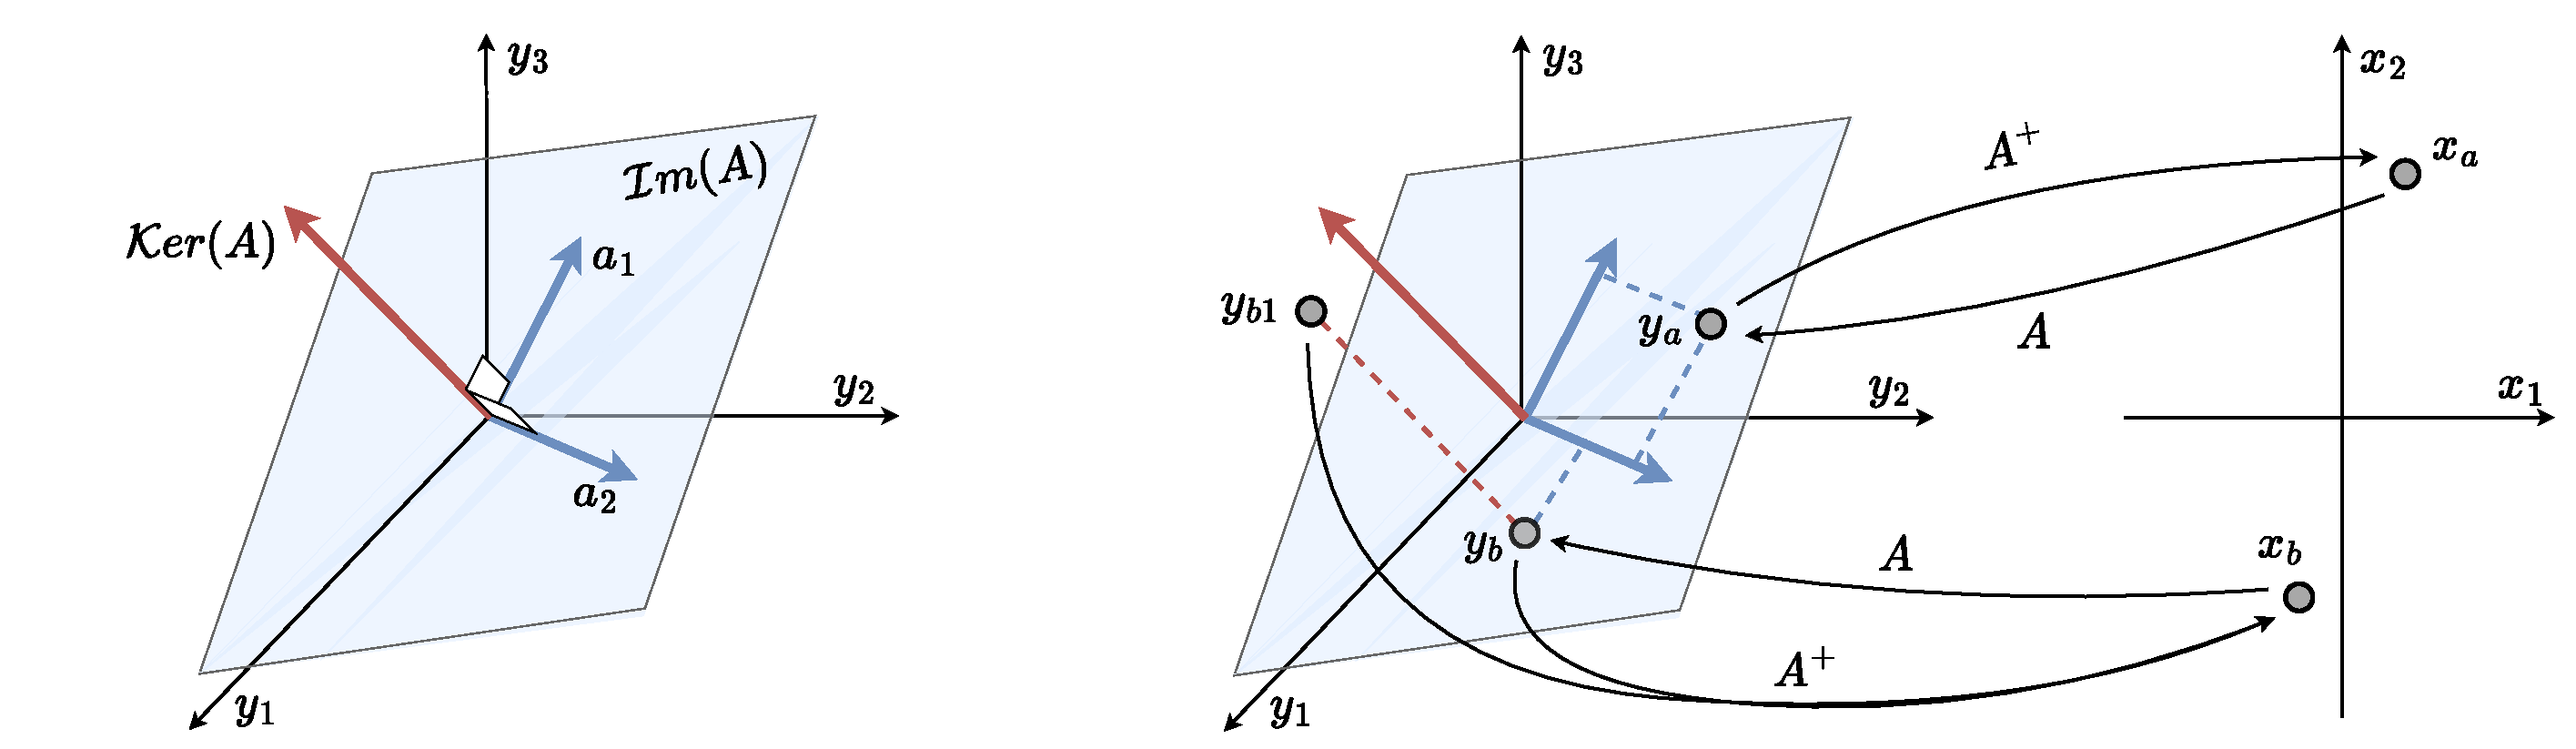
\includegraphics[width=\linewidth]{Chapters/imgs/pseudo_inverse_intuition_aio.pdf}
    \caption{Caption}
    \label{fig:pseudoinverse_intuition}
\end{figure}

The vectors $\bm{y}$, described by this matrix equation $\bm{y} = A\bm{x}$, form an $m$ dimensional subspace within the space $\bm{y}\in\mathbb{R}^n$, called the image $\img{\cdot}$ of the matrix $A$. 
\begin{equation}
    \bm{y}=A\bm{x} \in \img{A}
\end{equation}
Within the image $\img{A}$, the vectors $\bm{y}$ can be expressed as a linear combination of $m$ line vectors $\bm{a}_i\in\mathbb{R}^n$ of the matrix $A$ \cite{LARSON2013}
\begin{equation}
    \bm{y} = \bm{a}_1x_1 +  \bm{a}_2x_2 + \ldots +  \bm{a}_mx_m
\end{equation}
where $x_i$ are the scalar components of the vector $\bm{x}$.

% \begin{wrapfigure}{r}{0.6\linewidth}
%     \centering
%     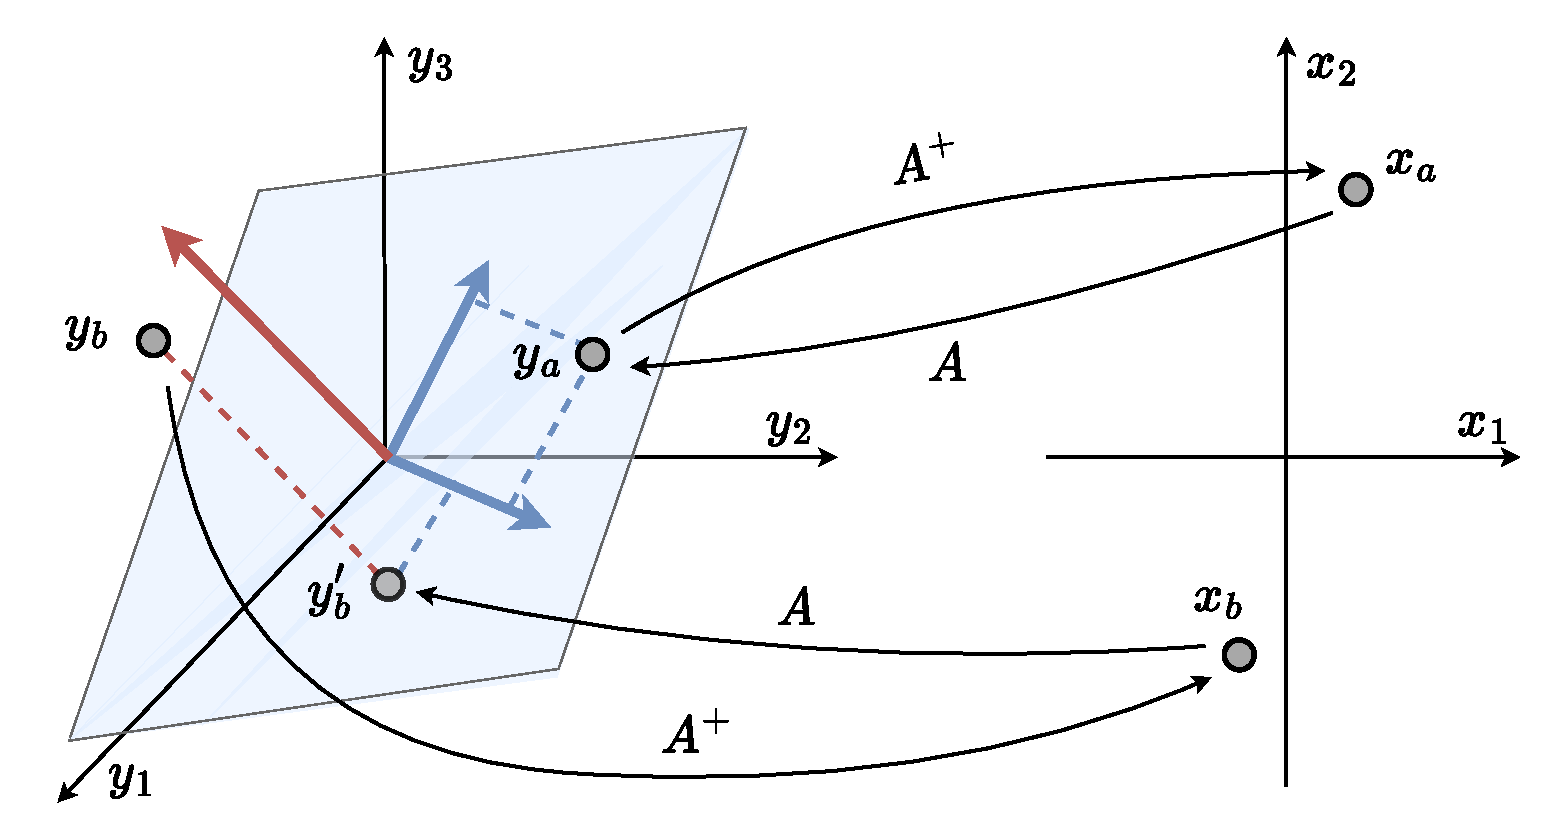
\includegraphics[width=\linewidth]{Chapters/imgs/pseudo_inverse_intuition.pdf}
%     \caption{Caption}
%     \label{fig:pseudoinverse_intuition}
% \end{wrapfigure}

Orthogonal to the $m$ dimensional image $\img{A}$, is the $n-m$ dimensional \textit{Null-space} or \textit{Kernel} space of the matrix $\ker{A}$. Together, the image $\img{A}$ and the $\ker{A}$, span the entire space of $\bm{y}\in\mathbb{R}^n$.
Figure \ref{fig:pseudoinverse_intuition} shows a visual example of the image and the null-space construction on for the space dimensions $n=3$ and $m=2$.

In general case, the vector $\bm{y}$ has components both in the image $\img{A}$ and the Null-space $\ker{A}$ of the matrix $A$
\begin{equation}
    \bm{y} = \bm{y}_i + \bm{y}_n, \quad \bm{y}_i\in\img{A}, \quad  \bm{y}_n\in\ker{A}
\end{equation}

When the vector $\bm{y}$ contains both image and null-space components, $\bm{y} = \bm{y}_i + \bm{y}_n$, the pseudo-inverse solution $\bm{x}_o = A^+\bm{y}$ and the corresponding vector $\bm{y}_o = A\bm{x}_o$, represents the solution with the minimum Euclidean distance $||\bm{y}_o - \bm{y}||^2$. As $\bm{y}$ can not be represented by $\bm{y}=A\bm{x}$, the minimal distance is not zero, indicating that $\bm{y}_o$ is not equal to $\bm{y}$. Geometrically, the solution $\bm{x}_o$ represents the vector $\bm{y}_o$ belonging to the image $\img{A}$ that is closest to $\bm{y}$ in terms of Euclidean distance. The vector $\bm{y}_o$ with the minimum distance to $\bm{y}$ corresponds to the image component $\bm{y}_i$
\begin{equation}
\bm{y}_i = \bm{y}_o= A\bm{x}_o = AA^+\bm{y}=AA^+(\bm{y}_i + \bm{y}_n)
\end{equation}
Meanwhile, the minimal distance corresponds to the null-space component $\bm{y}_n$
\begin{equation}
||\bm{A}\bm{x}_o - \bm{y}|| = ||\underbrace{AA^+\bm{y}}_{\bm{y}_i} ~~ - \bm{y}_i - \bm{y}_n ||= ||\bm{y}_n ||
\end{equation}

However, when the vector $\bm{y}$ consists of only image components $\bm{y}_i$, it can be represented as $\bm{y} = A\bm{x}$. In this case, the pseudo-inverse yields the solution $\bm{x}_o = A^+\bm{y}$, resulting in the vector $\bm{y}_o = A\bm{x}_o$ that is exactly equal to $\bm{y}$
\begin{equation}
\bm{y}_o-\bm{y} = A\bm{x}_o -\bm{y} = AA^+\bm{y} - \bm{y} =\bm{0}, \quad \forall\bm{y}\in\img{A}
\end{equation}

Therefore, the $\bm{x}_o$, obtained using the pseudo-inverse $\bm{x}_o=A^+\bm{y}$, can be used to generate the original vector $\bm{y} = A\bm{x}_o$, only if the original $\bm{y}$ belongs to the image $\img{A}$ of the matrix $A$. 


\todos{Finish!}

\section{Characterising the image space}
\label{ch:image_char}

As discussed in previous section, for any given vector $\bm{y} = \bm{y}_i + \bm{y}_n\in\mathbb{R}^n$, being composed of the image component $\bm{y}_i\in\img{A}$ and the null-space component $\bm{y}_n\in\ker{A}$, the image component $\bm{y}_i$ can be extracted using 
\begin{equation}
    \bm{y}_i =  AA^+\bm{y}
\end{equation}
where the matrix $AA^+$ represents the projector to the image $\img{A}$ \cite[p. 430]{meyer2001Matrix}. Its orthogonal projector, to the null-space $\ker{A}$, can be expressed as $I_{n\times n} - AA^+$, therefore the null-space component of $\bm{y}$ can be found using
\begin{equation}
    \bm{y}_n = (I_{n\times n} - AA^+)\bm{y}
\end{equation}

As all the vectors $\bm{y}$ belonging to the image $\img{A}$ have the null-space component equal to zero $\bm{y}_n=\bm{0}$, this relationship is commonly exploited to characterise the image space $\img{A}$
\begin{equation}
   \img{A} = \{ \bm{y}\in\mathbb{R}^n ~|~(I_{n\times n} - AA^+)\bm{y} = \bm{0}, \quad \bm{y}\in\mathbb{R}^n \}
   \label{eq:image_poly}
\end{equation}

This set, corresponding to the image space $\img{A}$, is particularly useful when it comes to characterising different intersection polytope formulations, as described in section \ref{ch:inter_formulaiton}.

\todos{SVD extension!}